\documentclass[12pt]{article}
\usepackage{amsmath}
\usepackage{amssymb}
\usepackage[table]{xcolor}
\usepackage{tikz}
\usepackage[margin=1in]{geometry}
\usepackage{blkarray}
\usepackage{graphicx}
\usepackage[colorlinks=true, linkcolor=blue, bookmarks=true, bookmarksopen=true]{hyperref}
\usepackage{float}
\usepackage[american]{circuitikz}
\usepackage{booktabs}
\usetikzlibrary{decorations.pathmorphing, patterns, arrows, calc}
\usetikzlibrary{shapes, arrows.meta, positioning, calc}
\title{Module 1: Mathematical Modeling of Control Systems}
\begin{document}
\maketitle

\section{Introduction}
A control system is a system that controls itself or other systems. It is defined as a device or set of devices to manage, command, direct, or regulate the behaviour of another system.

\vspace{0.5cm}
\begin{center}
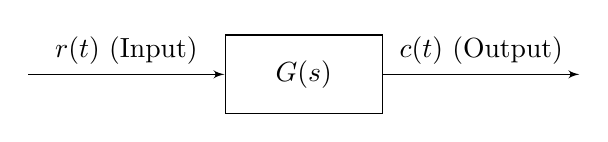
\begin{tikzpicture}[auto, node distance=3.5cm,>=latex']
    \node [coordinate] (input) {};
    \node [draw, rectangle, minimum height=1cm, minimum width=2cm, right of=input] (plant) {$G(s)$};
    \node [coordinate, right of=plant, node distance=3.5cm] (output) {};
    
    \draw [->] (input) -- node {$r(t)$ (Input)} (plant);
    \draw [->] (plant) -- node {$c(t)$ (Output)} (output);
\end{tikzpicture}
\end{center}
\vspace{0.5cm}

\section{Modeling of Electrical Systems}
The basic modeling variables for electrical systems are resistors, capacitors, and inductors.
\begin{itemize}
    \item \textbf{Resistor ($R$):} $v = iR$, $i = \dfrac{v}{R}$.
    \item \textbf{Capacitor ($C$):} $v = \dfrac{1}{C} \int i \, dt$, $i = C \dfrac{dv}{dt}$.
    \item \textbf{Inductor ($L$):} $v = L \dfrac{di}{dt}$, $i = \dfrac{1}{L} \int v \, dt$.
\end{itemize}

\subsubsection*{Example: Two-Loop RC Circuit}
To find the transfer function $G(s) = \dfrac{V_2(s)}{E(s)}$:

\vspace{0.5cm}
\begin{center}
\begin{circuitikz}
    \draw (0,0) to[V, l=$e(t)$] (0,3)
          to[R, l=$R_1$, i=$i_1$] (3,3)
          to[C, l=$C_1$, v=$v_1$] (3,0) -- (0,0);
    \draw (3,3) to[R, l=$R_2$, i=$i_2$] (6,3)
          to[C, l=$C_2$, v=$v_2$] (6,0) -- (3,0);
\end{circuitikz}
\end{center}
\vspace{0.5cm}
\setlength{\parindent}{0pt}
\textbf{Node 1 Equation:}
$i_1 + i_2 + i_3 = 0$.
\[ \frac{v_1 - e(t)}{R_1} + \frac{v_1 - v_2}{R_2} + C_1 \frac{dv_1}{dt} = 0  \]
Taking the Laplace transform:
\[ \frac{V_1(s) - E(s)}{R_1} + \frac{V_1(s) - V_2(s)}{R_2} + sC_1 V_1(s) = 0  \]

\textbf{Node 2 Equation:}
$i_1 + i_2 = 0$.
\[ \frac{v_2 - v_1}{R_2} + C_1 \frac{dv_2}{dt} = 0  \]
Taking the Laplace transform:
\[ V_2(s) \left[ \frac{1}{R_2} + sC_1 \right] = \frac{V_1(s)}{R_2} \implies V_1(s) = V_2(s)(1 + sR_2C_1)  \]

Substituting $V_1(s)$ into the first node equation yields the overall transfer function:
\[ H(s) = \dfrac{V_2(s)}{E(s)} = \dfrac{1}{(1 + sR_2C_1)\left(1 + \dfrac{R_1}{R_2} + sR_1C_1\right) - \dfrac{R_1}{R_2}}  \]

\section{Modeling of Mechanical Translational Systems}
The fundamental parameters of mechanical translational systems are mass ($m$), spring ($k$), and dashpot/damper ($B$).

\begin{itemize}
    \item \textbf{Mass:} Opposes acceleration. $F_m = m \dfrac{d^2x}{dt^2}$.
    \item \textbf{Spring:} Opposes displacement. $F_k = kx$.
    \item \textbf{Dashpot (Damper):} Opposes velocity. $F_B = Bv = B \dfrac{dx}{dt}$.
\end{itemize}

By force balance on a mass experiencing an external force $F$:
\[ F - f_m - f_k - f_B = 0  \]
\[ F = m\dfrac{d^2x}{dt^2} + B\dfrac{dx}{dt} + kx  \]

\vspace{0.5cm}
\begin{center}
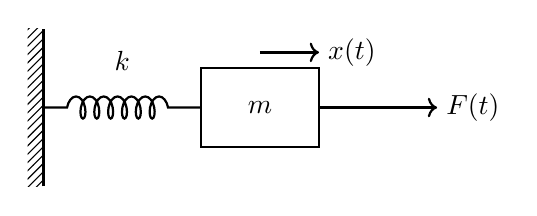
\begin{tikzpicture}[every node/.style={outer sep=0pt}]
    % Wall
    \fill[pattern=north east lines] (-0.2,-1) rectangle (0,1);
    \draw[thick] (0,-1) -- (0,1);
    
    % Mass
    \draw[thick] (2,-0.5) rectangle (3.5,0.5) node[midway] {$m$};
    
    % Spring
    \draw[thick, decoration={coil, amplitude=4pt, segment length=5pt, pre length=0.3cm, post length=0.3cm}, decorate] (0,0) -- (2,0) node[midway, above=10pt] {$k$};
    
    % Force arrow
    \draw[thick, ->] (3.5,0) -- (5,0) node[right] {$F(t)$};
    
    % Displacement arrow
    \draw[thick, ->] (2.75,0.7) -- (3.5,0.7) node[right] {$x(t)$};
\end{tikzpicture}
\end{center}


\section{Force-Voltage and Force-Current Analogies}
Electrical and mechanical systems share similar mathematical models represented by differential equations. We can map mechanical components to electrical components to create analogous circuits.

\begin{table}[h]
\centering
\begin{tabular}{@{}lll@{}}
\toprule
\textbf{Mechanical Translation} & \textbf{Force-Voltage (Mesh)} & \textbf{Force-Current (Nodal)} \\ \midrule
Force ($F$)                     & Voltage ($V$)                 & Current ($I$)                  \\
Mass ($m$)                      & Inductance ($L$)              & Capacitance ($C$)              \\
Spring constant ($k$)           & Elastance ($1/C$)             & Reciprocal Inductance ($1/L$)  \\
Damper ($B$)                    & Resistance ($R$)              & Conductance ($1/R$)            \\
Velocity ($v$)                  & Current ($i$)                 & Voltage ($v$)                  \\
Displacement ($x$)              & Charge ($q$)                  & Flux linkage ($\phi$)          \\ \bottomrule
\end{tabular}
\caption{Analogous Quantities }
\end{table}

\subsubsection*{Example System Analysis}
Consider a two-mass mechanical system:

\vspace{0.5cm}
\begin{center}
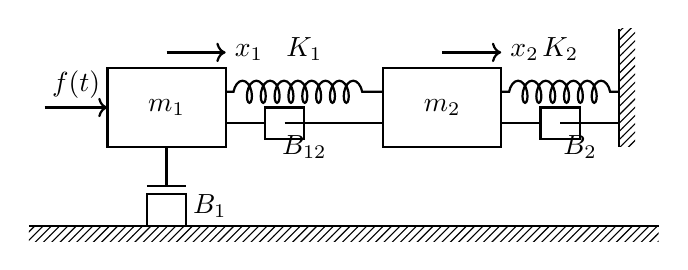
\begin{tikzpicture}[every node/.style={outer sep=0pt}, thick]
    % Ground
    \fill[pattern=north east lines] (0,-1) rectangle (8,-1.2);
    \draw (0,-1) -- (8,-1);

    % Mass 1
    \draw (1,0) rectangle (2.5,1) node[midway] {$m_1$};
    \draw[->] (0.2,0.5) -- (1,0.5) node[midway, above] {$f(t)$};
    \draw[->] (1.75, 1.2) -- (2.5, 1.2) node[right] {$x_1$};
    % Damper B1 to ground
    \draw (1.75,0) -- (1.75,-0.5);
    \draw (1.5,-0.5) -- (2,-0.5);
    \draw (1.5,-1) -- (1.5,-0.6) -- (2,-0.6) -- (2,-1);
    \node at (2.3, -0.75) {$B_1$};

    % Connecting Spring K1 and Damper B12
    \draw[decoration={coil, amplitude=4pt, segment length=5pt, pre length=0.1cm, post length=0.1cm}, decorate] (2.5,0.7) -- (4.5,0.7) node[midway, above=8pt] {$K_1$};
    \draw (2.5,0.3) -- (3,0.3);
    \draw (3,0.1) rectangle (3.5,0.5);
    \draw (3.25, 0.3) -- (4.5, 0.3);
    \node at (3.5, 0.0) {$B_{12}$};

    % Mass 2
    \draw (4.5,0) rectangle (6,1) node[midway] {$m_2$};
    \draw[->] (5.25, 1.2) -- (6, 1.2) node[right] {$x_2$};

    % Spring K2 and Damper B2 to wall
    \fill[pattern=north east lines] (7.5,0) rectangle (7.7,1.5);
    \draw (7.5,0) -- (7.5,1.5);
    \draw[decoration={coil, amplitude=4pt, segment length=5pt, pre length=0.1cm, post length=0.1cm}, decorate] (6,0.7) -- (7.5,0.7) node[midway, above=8pt] {$K_2$};
    
    \draw (6,0.3) -- (6.5,0.3);
    \draw (6.5,0.1) rectangle (7,0.5);
    \draw (6.75, 0.3) -- (7.5, 0.3);
    \node at (7, 0.0) {$B_2$};
\end{tikzpicture}
\end{center}
\vspace{0.2cm}

By applying force balance equations for both masses, we get following differential equations:

For Mass 1 ($m_1$):
\[ f(t) = m_1 \frac{d^2x_1}{dt^2} + B_1 \frac{dx_1}{dt} + K_1(x_1 - x_2) + B_{12} \frac{d(x_1 - x_2)}{dt} \text{ } \]

For Mass 2 ($m_2$):
\[ 0 = m_2 \frac{d^2x_2}{dt^2} + K_2 x_2 + B_2 \frac{dx_2}{dt} + K_1(x_2 - x_1) + B_{12} \frac{d(x_2 - x_1)}{dt} \text{ } \]



\subsubsection*{Force-Voltage Analogous Circuit}
Using the analogy $f(t) \rightarrow e(t)$ and $v \rightarrow i(t)$ (velocities $\dot{x}_1, \dot{x}_2$ become mesh currents $i_1, i_2$), we get following equations:

For Mesh 1:
\[ e(t) = L_1 \frac{di_1}{dt} + i_1 R_1 + \frac{1}{C_1} \int (i_1 - i_2) dt + R_{12}(i_1 - i_2) \]

\vspace{0.3cm}
\begin{center}
\begin{circuitikz}[scale=0.9]
    \draw (0,0) to[V, l=$e(t)$] (0,3)
          to[L, l=$L_1$] (2,3)
          to[R, l=$R_1$] (4,3);
    \draw (4,3) to[C, l=$C_1$] (4,1.5)
          to[R, l=$R_{12}$] (4,0);
    \draw (4,3) to[L, l=$L_2$] (6,3)
          to[C, l=$C_2$] (8,3)
          to[R, l=$R_2$] (8,0) -- (0,0);
    \draw (0,0) -- (4,0);
    
    \draw[thick, ->] (1.5,1.5) arc (150:-150:0.5) node[pos=0.5, right] {$i_1$};
    \draw[thick, ->] (5.5,1.5) arc (150:-150:0.5) node[pos=0.5, right] {$i_2$};
\end{circuitikz}
\end{center}
\vspace{0.2cm}

\subsubsection*{Force-Current Analogous Circuit}
Using the analogy $f(t) \rightarrow i(t)$ and $v \rightarrow v(t)$ (velocities $\dot{x}_1, \dot{x}_2$ become node voltages $v_1, v_2$):

\vspace{0.3cm}
\begin{center}
\begin{circuitikz}[scale=0.9]
    \draw (0,0) to[I, l=$i(t)$] (0,3) -- (1.5,3)
          to[R, l=$R_1$] (1.5,0) -- (0,0);
    \draw (1.5,3) -- (3,3) 
          to[C, l=$C_1$] (3,0) -- (1.5,0);
          
    % Parallel shared branch
    \draw (3,3) -- (3,4) to[L, l=$L_1$] (5,4) -- (5,3);
    \draw (3,3) to[R, l=$R_{12}$] (5,3);
    
    \draw (5,3) -- (6.5,3)
          to[C, l=$C_2$] (6.5,0) -- (3,0);
    \draw (6.5,3) -- (8,3)
          to[L, l=$L_2$] (8,0) -- (6.5,0);
    \draw (8,3) -- (9.5,3)
          to[R, l=$R_2$] (9.5,0) -- (8,0);
          
    \node at (3,3.3) {$v_1$};
    \node at (5,3.3) {$v_2$};
\end{circuitikz}
\end{center}
\vspace{0.2cm}

Node 1 Equation:
\[ i(t) = \frac{v_1}{R_1} + C_1 \frac{dv_1}{dt} + \frac{1}{L_1} \int (v_1 - v_2) dt + \frac{v_1 - v_2}{R_{12}} \]

\subsection*{5. Complex Mechanical Systems (3-DOF)}
For a system with three masses ($m_1, m_2, m_3$) connected in sequence, you follow the same rules by establishing a reference node for each mass displacement ($x_1, x_2, x_3$).

The differential equations take the form:
\begin{align*}
    m_1 \frac{d^2x_1}{dt^2} + B_1 \frac{dx_1}{dt} + K_1 x_1 + K_2(x_1 - x_2) &= f_1(t) \\
    m_2 \frac{d^2x_2}{dt^2} + B_2 \frac{d(x_2 - x_3)}{dt} + K_2(x_2 - x_1) + K_3(x_2 - x_3) &= f_2(t) \\
    m_3 \frac{d^2x_3}{dt^2} + B_2 \frac{d(x_3 - x_2)}{dt} + K_3(x_3 - x_2) &= 0
\end{align*}

When drawing the equivalent circuits, the number of meshes (for Force-Voltage) or the number of principal nodes (for Force-Current) exactly equals the number of masses in the mechanical system.


\tikzstyle{block} = [draw, rectangle, minimum height=3em, minimum width=4em]
\tikzstyle{sum} = [draw, circle, node distance=1.5cm]
\tikzstyle{input} = [coordinate]
\tikzstyle{output} = [coordinate]
\tikzstyle{branch} = [fill, shape=circle, minimum size=3pt, inner sep=0pt]


\section{Open Loop vs. Closed Loop Control Systems}

\subsection{Open Loop Control System}
A system in which the control action is entirely independent of the output. The output has no effect on the control action. 
\begin{itemize}
    \item \textbf{Advantages:} Simple construction, economical, usually stable, and easy to maintain.
    \item \textbf{Disadvantages:} Inaccurate, highly sensitive to parameter changes, and easily affected by external disturbances.
\end{itemize}

\subsubsection*{Closed Loop Control System}
A system equipped with an error detector that automatically corrects changes in the output by adjusting the input. Feedback is continuously present.
\begin{itemize}
    \item \textbf{Advantages:} Highly accurate, suppresses external disturbances, and provides a speedy response.
    \item \textbf{Disadvantages:} Complex, expensive, requires high maintenance, and is prone to instability or oscillations.
\end{itemize}

\begin{table}[h]
\centering
\begin{tabular}{@{}ll@{}}
\toprule
\textbf{Open Loop System} & \textbf{Closed Loop System} \\ \midrule
No feedback present  & Feedback is present  \\
Inaccurate  & Accurate  \\
Highly sensitive to parameter changes  & Less sensitive to parameter changes  \\
Stable  & May become unstable  \\
Simple construction \& economical  & Complicated \& costlier  \\
Examples: Fan, automatic toaster  & Examples: AC, missile launcher  \\ \bottomrule
\end{tabular}
\caption{Comparison of Control Systems}
\end{table}

\subsection*{2. Closed Loop Transfer Function}
For a standard closed-loop system with forward path gain $G(s)$ and feedback path gain $H(s)$:
\[ E(s) = R(s) - H(s)C(s) \text{  } \]
\[ C(s) = G(s)E(s) = G(s)[R(s) - H(s)C(s)] \text{  } \]
\[ C(s)[1 + G(s)H(s)] = G(s)R(s) \implies \frac{C(s)}{R(s)} = \frac{G(s)}{1 + G(s)H(s)} \text{  } \]

\subsection{Rules for Block Diagram Reduction}

\tikzset{
    block/.style = {draw, rectangle, minimum height=2.5em, minimum width=3.5em},
    sum/.style = {draw, circle, inner sep=1pt, minimum size=1.5em},
    branch/.style = {fill, shape=circle, minimum size=3pt, inner sep=0pt},
    input/.style = {coordinate},
    output/.style = {coordinate},
    >=Stealth
}



\subsection*{1. Combining Blocks in Cascade}
% Rule 1: Cascade 
\begin{tikzpicture}[auto, node distance=2cm]
    \node [input] (in) {};
    \node [block, right of=in, node distance=1.5cm] (g1) {$G_1$};
    \node [block, right of=g1] (g2) {$G_2$};
    \node [output, right of=g2, node distance=1.5cm] (out) {};
    
    \draw [->] (in) -- node {$A$} (g1);
    \draw [->] (g1) -- (g2);
    \draw [->] (g2) -- node {$AG_1G_2$} (out);
    
    \node [right of=out, node distance=1cm] (eq) {$\equiv$};
    
    \node [input, right of=eq, node distance=1cm] (in2) {};
    \node [block, right of=in2, node distance=2cm] (g12) {$G_1 G_2$};
    \node [output, right of=g12, node distance=2cm] (out2) {};
    
    \draw [->] (in2) -- node {$A$} (g12);
    \draw [->] (g12) -- node {$AG_1G_2$} (out2);
\end{tikzpicture}

\subsection*{2. Combining Blocks in Parallel}
% Rule 2: Parallel 
\begin{tikzpicture}[auto, node distance=1.5cm]
    \node [input] (in) {};
    \node [branch, right of=in, node distance=1cm] (br) {};
    \node [block, above right=0.5cm and 1cm of br] (g1) {$G_1$};
    \node [block, below right=0.5cm and 1cm of br] (g2) {$G_2$};
    \node [sum, right=2.5cm of br] (sum) {$\Sigma$};
    \node [output, right of=sum, node distance=1.5cm] (out) {};
    
    \draw [->] (in) -- node {$A$} (br);
    \draw [->] (br) |- (g1);
    \draw [->] (br) |- (g2);
    \draw [->] (g1) -| node[pos=0.9, right] {$+$} (sum);
    \draw [->] (g2) -| node[pos=0.9, right] {$+$} (sum);
    \draw [->] (sum) -- node {$A(G_1+G_2)$} (out);
    
    \node [right of=out, node distance=1cm] (eq) {$\equiv$};
    
    \node [input, right of=eq, node distance=1cm] (in2) {};
    \node [block, right of=in2, node distance=2cm] (g12) {$G_1 + G_2$};
    \node [output, right of=g12, node distance=2cm] (out2) {};
    
    \draw [->] (in2) -- node {$A$} (g12);
    \draw [->] (g12) -- node {$A(G_1+G_2)$} (out2);
\end{tikzpicture}

\vspace{0.5cm}
\subsection*{3. Moving a Branch Point After a Block}
% Rule 3: Branch after block 
\begin{tikzpicture}[auto, node distance=2cm]
    \node [input] (in) {};
    \node [branch, right of=in, node distance=1.5cm] (br) {};
    \node [block, right of=br, node distance=1.5cm] (g) {$G$};
    \node [output, right of=g, node distance=1.5cm] (out) {};
    \node [output, below of=br, node distance=1.2cm] (out_br) {};
    
    \draw [->] (in) -- node {$A$} (br);
    \draw [->] (br) -- (g);
    \draw [->] (g) -- node {$AG$} (out);
    \draw [->] (br) -- node[right] {$A$} (out_br);
    
    \node [right of=out, node distance=1cm] (eq) {$\equiv$};
    
    \node [input, right of=eq, node distance=1cm] (in2) {};
    \node [block, right of=in2, node distance=1.5cm] (g2) {$G$};
    \node [branch, right of=g2, node distance=1.5cm] (br2) {};
    \node [output, right of=br2, node distance=1.5cm] (out2) {};
    \node [block, below of=br2, node distance=1.2cm] (ginv) {$1/G$};
    \node [output, left of=ginv, node distance=1.5cm] (out_br2) {};
    
    \draw [->] (in2) -- node {$A$} (g2);
    \draw [->] (g2) -- (br2);
    \draw [->] (br2) -- node {$AG$} (out2);
    \draw [->] (br2) -- (ginv);
    \draw [->] (ginv) -- node[above] {$A$} (out_br2);
\end{tikzpicture}

\vspace{0.5cm}
\subsection*{4. Moving a Branch Point Before a Block}
% Rule 4: Branch before block 
\begin{tikzpicture}[auto, node distance=2cm]
    \node [input] (in) {};
    \node [block, right of=in, node distance=1.5cm] (g) {$G$};
    \node [branch, right of=g, node distance=1.5cm] (br) {};
    \node [output, right of=br, node distance=1.5cm] (out) {};
    \node [output, below of=br, node distance=1.2cm] (out_br) {};
    
    \draw [->] (in) -- node {$A$} (g);
    \draw [->] (g) -- (br);
    \draw [->] (br) -- node {$AG$} (out);
    \draw [->] (br) -- node[right] {$AG$} (out_br);
    
    \node [right of=out, node distance=1cm] (eq) {$\equiv$};
    
    \node [input, right of=eq, node distance=1cm] (in2) {};
    \node [branch, right of=in2, node distance=1.5cm] (br2) {};
    \node [block, right of=br2, node distance=1.5cm] (g2) {$G$};
    \node [output, right of=g2, node distance=1.5cm] (out2) {};
    \node [block, below of=g2, node distance=1.2cm] (g3) {$G$};
    \node [output, right of=g3, node distance=1.5cm] (out_br2) {};
    
    \draw [->] (in2) -- node {$A$} (br2);
    \draw [->] (br2) -- (g2);
    \draw [->] (g2) -- node {$AG$} (out2);
    \draw [->] (br2) |- (g3);
    \draw [->] (g3) -- node[above] {$AG$} (out_br2);
\end{tikzpicture}

\vspace{0.5cm}
\subsection*{5. Moving a Summing Point After a Block}
% Rule 5: Summing point after block 
\begin{tikzpicture}[auto, node distance=2cm]
    \node [input] (in) {};
    \node [sum, right of=in, node distance=1.5cm] (sum) {$\Sigma$};
    \node [input, below of=sum, node distance=1cm] (in_b) {};
    \node [block, right of=sum, node distance=1.5cm] (g) {$G$};
    \node [output, right of=g, node distance=2cm] (out) {};
    
    \draw [->] (in) -- node {$A$} (sum);
    \draw [->] (in_b) -- node[right] {$B$} (sum);
    \draw [->] (sum) -- (g);
    \draw [->] (g) -- node {$G(A+B)$} (out);
    
    \node [right of=out, node distance=0.5cm] (eq) {$\equiv$};
    
    \node [input, right of=eq, node distance=1cm] (in2) {};
    \node [block, right of=in2, node distance=1.5cm] (g2) {$G$};
    \node [sum, right of=g2, node distance=1.5cm] (sum2) {$\Sigma$};
    \node [output, right of=sum2, node distance=1.5cm] (out2) {};
    \node [block, below of=g2, node distance=1.2cm] (g3) {$G$};
    \node [input, left of=g3, node distance=1.5cm] (in_b2) {};
    
    \draw [->] (in2) -- node {$A$} (g2);
    \draw [->] (g2) -- (sum2);
    \draw [->] (in_b2) -- node {$B$} (g3);
    \draw [->] (g3) -| (sum2);
    \draw [->] (sum2) -- node {$AG+BG$} (out2);
\end{tikzpicture}

\vspace{0.5cm}
\subsection*{6. Moving a Summing Point Before a Block}
% Rule 6: Summing point before block 
\begin{tikzpicture}[auto, node distance=2cm]
    \node [input] (in) {};
    \node [block, right of=in, node distance=1.5cm] (g) {$G$};
    \node [sum, right of=g, node distance=1.5cm] (sum) {$\Sigma$};
    \node [input, below of=sum, node distance=1cm] (in_b) {};
    \node [output, right of=sum, node distance=1.5cm] (out) {};
    
    \draw [->] (in) -- node {$A$} (g);
    \draw [->] (g) -- (sum);
    \draw [->] (in_b) -- node[right] {$B$} (sum);
    \draw [->] (sum) -- node {$AG+B$} (out);
    
    \node [right of=out, node distance=1cm] (eq) {$\equiv$};
    
    \node [input, right of=eq, node distance=1cm] (in2) {};
    \node [sum, right of=in2, node distance=1.5cm] (sum2) {$\Sigma$};
    \node [block, right of=sum2, node distance=1.5cm] (g2) {$G$};
    \node [output, right of=g2, node distance=2cm] (out2) {};
    \node [block, below of=sum2, node distance=1.2cm] (ginv) {$1/G$};
    \node [input, left of=ginv, node distance=1.5cm] (in_b2) {};
    
    \draw [->] (in2) -- node {$A$} (sum2);
    \draw [->] (sum2) -- (g2);
    \draw [->] (g2) -- node {$G(A+B/G)$} (out2);
    \draw [->] (in_b2) -- node {$B$} (ginv);
    \draw [->] (ginv) -- (sum2);
\end{tikzpicture}

\subsection*{7. Interchanging Summing Points}
Consecutive summing points can be swapped without affecting the final output .

\vspace{0.3cm}
\begin{center}
\begin{tikzpicture}[auto, node distance=2cm]
    % Left side
    \node [input] (in) {};
    \node [sum, right of=in, node distance=1.5cm] (sum1) {$\Sigma$};
    \node [input, below of=sum1, node distance=1.2cm] (inB) {};
    \node [sum, right of=sum1, node distance=1.5cm] (sum2) {$\Sigma$};
    \node [input, below of=sum2, node distance=1.2cm] (inC) {};
    \node [output, right of=sum2, node distance=2cm] (out) {};
    
    \draw [->] (in) -- node {$A$} (sum1);
    \draw [->] (inB) -- node[right] {$+$} node[near start, right] {$B$} (sum1);
    \draw [->] (sum1) -- (sum2);
    \draw [->] (inC) -- node[right] {$-$} node[near start, right] {$C$} (sum2);
    \draw [->] (sum2) -- node {$A+B-C$} (out);
    
    \node [right of=out, node distance=0.5cm] (eq) {$\equiv$};
    
    % Right side
    \node [input, right of=eq, node distance=1cm] (in2) {};
    \node [sum, right of=in2, node distance=1.5cm] (sum3) {$\Sigma$};
    \node [input, below of=sum3, node distance=1.2cm] (inC2) {};
    \node [sum, right of=sum3, node distance=1.5cm] (sum4) {$\Sigma$};
    \node [input, below of=sum4, node distance=1.2cm] (inB2) {};
    \node [output, right of=sum4, node distance=2cm] (out2) {};
    
    \draw [->] (in2) -- node {$A$} (sum3);
    \draw [->] (inC2) -- node[right] {$-$} node[near start, right] {$C$} (sum3);
    \draw [->] (sum3) -- (sum4);
    \draw [->] (inB2) -- node[right] {$+$} node[near start, right] {$B$} (sum4);
    \draw [->] (sum4) -- node {$A-C+B$} (out2);
\end{tikzpicture}
\end{center}

\vspace{0.5cm}
\subsection*{10. Combining / Splitting Summing Points}
Two or more summing points connected directly in cascade can be combined into a single summing point, and a single multi-input summing point can be split into two or more separate summing points .

\vspace{0.3cm}
\begin{center}
\begin{tikzpicture}[auto, node distance=2cm]
    % Left side: Two summing points (Splitted)
    \node [input] (inA) {};
    \node [sum, right of=inA, node distance=1.5cm] (sum1) {$\Sigma$};
    \node [input, below of=sum1, node distance=1.2cm] (inB) {};
    \node [sum, right of=sum1, node distance=1.5cm] (sum2) {$\Sigma$};
    \node [input, below of=sum2, node distance=1.2cm] (inC) {};
    \node [output, right of=sum2, node distance=2cm] (out1) {};
    
    \draw [->] (inA) -- node {$A$} (sum1);
    \draw [->] (inB) -- node[right] {$+$} node[near start, right] {$B$} (sum1);
    \draw [->] (sum1) -- (sum2);
    \draw [->] (inC) -- node[right] {$-$} node[near start, right] {$C$} (sum2);
    \draw [->] (sum2) -- node {$A+B-C$} (out1);
    
    \node [right of=out1, node distance=0.5cm] (eq) {$\equiv$};
    
    % Right side: One combined summing point
    \node [input, right of=eq, node distance=1.5cm] (inA2) {};
    \node [sum, right of=inA2, node distance=1.5cm] (sum3) {$\Sigma$};
    \node [input, above of=sum3, node distance=1.2cm] (inB2) {};
    \node [input, below of=sum3, node distance=1.2cm] (inC2) {};
    \node [output, right of=sum3, node distance=2cm] (out2) {};
    
    \draw [->] (inA2) -- node {$A$} (sum3);
    \draw [->] (inB2) -- node[right] {$+$} node[near start, right] {$B$} (sum3);
    \draw [->] (inC2) -- node[right] {$-$} node[near start, right] {$C$} (sum3);
    \draw [->] (sum3) -- node {$A+B-C$} (out2);
\end{tikzpicture}
\end{center}

\subsection*{8. Elimination of Negative Feedback}
A standard negative feedback loop reduces to a single forward block divided by one plus the loop gain .

\vspace{0.3cm}
\begin{center}
\begin{tikzpicture}[auto, node distance=2cm]
    % Left side
    \node [input] (R) {};
    \node [sum, right of=R, node distance=1.5cm] (sum) {$\Sigma$};
    \node [block, right of=sum, node distance=2cm] (G) {$G(s)$};
    \node [branch, right of=G, node distance=1.5cm] (br) {};
    \node [output, right of=br, node distance=1.5cm] (C) {};
    \node [block, below of=G, node distance=1.5cm] (H) {$H(s)$};
    
    \draw [->] (R) -- node {$R$} (sum);
    \draw [->] (sum) -- node {$E$} (G);
    \draw [->] (G) -- (br);
    \draw [->] (br) -- node {$C$} (C);
    \draw [->] (br) |- (H);
    \draw [->] (H) -| node[pos=0.9, right] {$-$} (sum);
    
    \node [right of=C, node distance=0.5cm] (eq) {$\equiv$};
    
    % Right side
    \node [input, right of=eq, node distance=1cm] (R2) {};
    \node [block, right of=R2, node distance=2.5cm] (Sys) {$\frac{G}{1+GH}$};
    \node [output, right of=Sys, node distance=2.5cm] (C2) {};
    
    \draw [->] (R2) -- node {$R$} (Sys);
    \draw [->] (Sys) -- node {$C$} (C2);
\end{tikzpicture}
\end{center}

\vspace{0.5cm}
\subsection*{9. Elimination of Positive Feedback}
A positive feedback loop reduces to a single forward block divided by one minus the loop gain .

\vspace{0.3cm}
\begin{center}
\begin{tikzpicture}[auto, node distance=2cm]
    % Left side
    \node [input] (R) {};
    \node [sum, right of=R, node distance=1.5cm] (sum) {$\Sigma$};
    \node [block, right of=sum, node distance=2cm] (G) {$G(s)$};
    \node [branch, right of=G, node distance=1.5cm] (br) {};
    \node [output, right of=br, node distance=1.5cm] (C) {};
    \node [block, below of=G, node distance=1.5cm] (H) {$H(s)$};
    
    \draw [->] (R) -- node {$R$} (sum);
    \draw [->] (sum) -- node {$E$} (G);
    \draw [->] (G) -- (br);
    \draw [->] (br) -- node {$C$} (C);
    \draw [->] (br) |- (H);
    \draw [->] (H) -| node[pos=0.9, right] {$+$} (sum);
    
    \node [right of=C, node distance=0.5cm] (eq) {$\equiv$};
    
    % Right side
    \node [input, right of=eq, node distance=1cm] (R2) {};
    \node [block, right of=R2, node distance=2.5cm] (Sys) {$\frac{G}{1-GH}$};
    \node [output, right of=Sys, node distance=2.5cm] (C2) {};
    
    \draw [->] (R2) -- node {$R$} (Sys);
    \draw [->] (Sys) -- node {$C$} (C2);
\end{tikzpicture}
\end{center}

\tikzset{
    block/.style = {draw, rectangle, minimum height=2.5em, minimum width=3.5em},
    sum/.style = {draw, circle, inner sep=1pt, minimum size=1.5em},
    branch/.style = {fill, shape=circle, minimum size=3pt, inner sep=0pt},
    input/.style = {coordinate},
    output/.style = {coordinate},
    >=Stealth
}


\subsection*{Example 1: Feedforward and Feedback Overlap}
\textbf{Problem:} Reduce the block diagram to find the closed-loop transfer function $\frac{C(s)}{R(s)}$.

\vspace{0.5cm}
\begin{center}
\begin{tikzpicture}[auto, node distance=2cm]
    \node [input] (R) {};
    \node [sum, right of=R, node distance=1.5cm] (S1) {$\Sigma$};
    \node [branch, right of=S1, node distance=1.2cm] (nodeA) {};
    \node [block, right of=nodeA, node distance=1.5cm] (G1) {$G_1$};
    \node [branch, right of=G1, node distance=1.5cm] (nodeB) {};
    \node [block, right of=nodeB, node distance=1.5cm] (G2) {$G_2$};
    \node [sum, right of=G2, node distance=1.5cm] (S2) {$\Sigma$};
    \node [output, right of=S2, node distance=1.5cm] (C) {};
    
    \node [block, above of=G1, node distance=1.5cm] (G3) {$G_3$};
    \node [block, below of=G1, node distance=1.5cm] (H) {$H$};
    
    \draw [->] (R) -- node {$R(s)$} (S1);
    \draw [-] (S1) -- node {$A$} (nodeA);
    \draw [->] (nodeA) -- (G1);
    \draw [->] (nodeA) |- (G3);
    \draw [-] (G1) -- (nodeB);
    \draw [->] (nodeB) -- (G2);
    \draw [->] (G2) -- node[pos=0.8, below] {$+$} (S2);
    \draw [->] (G3) -| node[pos=0.9, right] {$+$} (S2);
    \draw [->] (S2) -- node {$C(s)$} (C);
    
    \draw [->] (nodeB) |- (H);
    \draw [->] (H) -| node[pos=0.9, right] {$-$} (S1);
\end{tikzpicture}
\end{center}

\textbf{Solution:}
Let the signal after the first summing point be $A$. 
1. The inner feedback loop output is $A = R - H \cdot (G_1 A)$.
2. Solving for $A$: $A(1 + G_1 H) = R \implies A = \frac{R}{1 + G_1 H}$.
3. The output $C(s)$ is the sum of the feedforward path and the main path: 
   $$C = G_3 A + G_2(G_1 A) = A(G_1 G_2 + G_3)$$
4. Substituting $A$ into the output equation yields the transfer function:
   $$\frac{C(s)}{R(s)} = \frac{G_1 G_2 + G_3}{1 + G_1 H}$$

\vspace{1cm}

\subsection*{Example 2: Moving Pick-off Points}
\textbf{Problem:} Reduce the diagram with overlapping loops.

\vspace{0.5cm}
\begin{center}
\begin{tikzpicture}[auto, node distance=2cm]
    \node [input] (R) {};
    \node [branch, right of=R, node distance=1cm] (brR) {};
    \node [sum, right of=brR, node distance=1.2cm] (S1) {$\Sigma$};
    \node [block, right of=S1, node distance=1.5cm] (G1) {$G_1$};
    \node [sum, right of=G1, node distance=1.5cm] (S2) {$\Sigma$};
    \node [block, right of=S2, node distance=1.5cm] (G2) {$G_2$};
    \node [branch, right of=G2, node distance=1.2cm] (nodeX) {};
    \node [block, right of=nodeX, node distance=1.5cm] (G3) {$G_3$};
    \node [branch, right of=G3, node distance=1.2cm] (nodeY) {};
    \node [sum, right of=nodeY, node distance=1.5cm] (S3) {$\Sigma$};
    \node [output, right of=S3, node distance=1.5cm] (C) {};
    
    \node [block, below of=G2, node distance=1.5cm] (H1) {$H_1$};
    \node [block, above of=G2, node distance=1.5cm] (H2) {$H_2$};
    \node [block, below of=H1, node distance=1cm] (G4) {$G_4$};
    
    \draw [->] (R) -- node {$R(s)$} (S1);
    \draw [->] (S1) -- (G1);
    \draw [->] (G1) -- node[pos=0.8, below] {$+$} (S2);
    \draw [->] (S2) -- (G2);
    \draw [-] (G2) -- (nodeX);
    \draw [->] (nodeX) -- (G3);
    \draw [-] (G3) -- (nodeY);
    \draw [->] (nodeY) -- node[pos=0.8, below] {$+$} (S3);
    \draw [->] (S3) -- node {$C(s)$} (C);
    
    % H1 Feedback
    \draw [->] (nodeX) |- (H1);
    \draw [->] (H1) -| node[pos=0.9, right] {$-$} (S1);
    
    % H2 Feedback
    \draw [->] (nodeY) |- (H2);
    \draw [->] (H2) -| node[pos=0.9, left] {$-$} (S2);
    
    % G4 Feedforward
    \draw [->] (brR) |- (G4);
    \draw [->] (G4) -| node[pos=0.9, right] {$+$} (S3);
\end{tikzpicture}
\end{center}

\textbf{Solution:}
1. \textbf{Move pick-off point:} Move the pick-off point for $H_1$ from behind $G_3$ to ahead of $G_3$. To maintain the same signal, the feedback block $H_1$ becomes $\frac{H_1}{G_3}$.
2. \textbf{Resolve inner loop:} The loop with $G_2, G_3,$ and $H_2$ reduces to $A = \frac{G_2 G_3}{1 + G_2 G_3 H_2}$.
3. \textbf{Resolve outer loop:} The main forward path is now $G_1 A$, and the feedback is $\frac{H_1}{G_3}$. 
   This loop reduces to $B = \frac{G_1 A}{1 + G_1 A (\frac{H_1}{G_3})}$.
   Substituting $A$: 
   $$B = \frac{G_1 G_2 G_3}{1 + G_2 G_3 H_2 + G_1 G_2 H_1}$$
4. \textbf{Add feedforward:} The final output $C(s)$ sums the reduced main path $B$ and the feedforward path $G_4$.
   $$\frac{C(s)}{R(s)} = \frac{G_1 G_2 G_3}{1 + G_2 G_3 H_2 + G_1 G_2 H_1} + G_4$$

\vspace{1cm}

\subsection*{Example 3: Multiple Feedbacks with Input Feedforward}
\textbf{Problem:} Reduce the system containing an input feedforward and two global negative feedbacks.

\vspace{0.5cm}
\begin{center}
\begin{tikzpicture}[auto, node distance=2cm]
    \node [input] (R) {};
    \node [branch, right of=R, node distance=1cm] (brR) {};
    \node [sum, right of=brR, node distance=1.5cm] (S1) {$\Sigma$};
    \node [block, right of=S1, node distance=1.5cm] (G1) {$G_1$};
    \node [sum, right of=G1, node distance=1.5cm] (S2) {$\Sigma$};
    \node [block, right of=S2, node distance=1.5cm] (G2) {$G_2$};
    \node [branch, right of=G2, node distance=1.5cm] (brC1) {};
    \node [branch, right of=brC1, node distance=1cm] (brC2) {};
    \node [output, right of=brC2, node distance=1.5cm] (C) {};
    
    \node [block, below of=G1, node distance=1.5cm] (H2) {$H_2$};
    \node [block, below of=H2, node distance=1.2cm] (H1) {$H_1$};
    
    \draw [->] (R) -- node {$R(s)$} (S1);
    \draw [->] (S1) -- (G1);
    \draw [->] (G1) -- node[pos=0.8, below] {$+$} (S2);
    \draw [->] (S2) -- (G2);
    \draw [-] (G2) -- (brC1);
    \draw [-] (brC1) -- (brC2);
    \draw [->] (brC2) -- node {$C(s)$} (C);
    
    % R Feedforward to S2
    \draw [->] (brR) |- ++(0, 1.5) -| node[pos=0.9, right] {$+$} (S2);
    
    % C Feedback to S2 (via H2)
    \draw [->] (brC1) |- (H2);
    \draw [->] (H2) -| node[pos=0.9, right] {$-$} (S2);
    
    % C Feedback to S1 (via H1)
    \draw [->] (brC2) |- (H1);
    \draw [->] (H1) -| node[pos=0.9, right] {$-$} (S1);
\end{tikzpicture}
\end{center}

\textbf{Solution:}
Using algebraic equations to derive the transfer function without redrawing:
1. Equation at $S_1$: Output is $E_1 = R - H_1 C$.
2. The signal before $S_2$ is $G_1 E_1 = G_1(R - H_1 C)$.
3. Equation at $S_2$: Output is $E_2 = G_1(R - H_1 C) + R - H_2 C$.
4. The final output is $C = G_2 E_2$. Substituting $E_2$:
   $$C = G_2 [G_1(R - H_1 C) + R - H_2 C]$$
   $$C = G_1 G_2 R - G_1 G_2 H_1 C + G_2 R - G_2 H_2 C$$
5. Group all terms with $C$ on the left side:
   $$C (1 + G_1 G_2 H_1 + G_2 H_2) = R (G_2 + G_1 G_2)$$
6. The transfer function is therefore:
   $$\frac{C(s)}{R(s)} = \frac{G_2(1 + G_1)}{1 + G_2 H_2 + G_1 G_2 H_1}$$

\tikzset{
    node/.style={circle, fill=black, inner sep=1.5pt},
    >=Stealth
}


\section{Signal Flow Graphs (SFG)}

Developed by S. J. Mason, a Signal Flow Graph is a graphical representation of the simultaneous equations describing a system .
\begin{itemize}
    \item \textbf{Nodes:} Represent system variables (inputs, outputs, summing points, branch points) .
    \item \textbf{Branches:} Represent the transfer functions (gains) between nodes, drawn as directed lines or arcs .
\end{itemize}

\subsection{Mason's Gain Formula}
The overall transmittance (transfer function) $T$ from the input node to the output node is given by :
\[ T = \frac{1}{\Delta} \sum_{k} P_k \Delta_k \] 

Where:
\begin{itemize}
    \item $k = $ total number of forward paths .
    \item $P_k = $ path gain of the $k^{th}$ forward path .
    \item $\Delta = 1 - (\text{sum of all individual loop gains}) + (\text{sum of gain products of all possible combinations of 2 non-touching loops}) - (\text{sum of gain products of all possible combinations of 3 non-touching loops}) + \dots$ .
    \item $\Delta_k = $ the value of $\Delta$ for that part of the graph not touching the $k^{th}$ forward path .
\end{itemize}

\vspace{0.5cm}

\subsection{Example 1: Standard Closed-Loop System}
Converting a standard feedback block diagram to an SFG and solving it .

\vspace{0.5cm}
\begin{center}
\begin{tikzpicture}[auto, node distance=2.5cm]
    \node[node, label=below:1] (n1) {};
    \node[left of=n1, node distance=0.5cm] {$R(s)$};
    \node[node, right of=n1, label=below:2] (n2) {};
    \node[node, right of=n2, label=below:3] (n3) {};
    \node[node, right of=n3, label=below:4] (n4) {};
    \node[right of=n4, node distance=0.5cm] {$C(s)$};
    
    \draw[->] (n1) -- node {$1$} (n2);
    \draw[->] (n2) -- node {$G$} (n3);
    \draw[->] (n3) -- node {$1$} (n4);
    
    \draw[->] (n3) to[bend left=45] node {$-H$} (n2);
\end{tikzpicture}
\end{center}

\textbf{Solution:}
\begin{enumerate}
    \item \textbf{Forward Paths:} $k = 1$. The path gain is $P_1 = 1 \cdot G \cdot 1 = G$.
    \item \textbf{Individual Loops:} There is one loop with gain $L_1 = -GH$.
    \item \textbf{Non-touching Loops:} None (0).
    \item \textbf{Determinant $\Delta$:} $\Delta = 1 - (L_1) = 1 + GH$ .
    \item \textbf{Path Factor $\Delta_1$:} The forward path touches all nodes of the loop, so $\Delta_1 = 1 - 0 = 1$.
\end{enumerate}
\[ T = \frac{P_1 \Delta_1}{\Delta} = \frac{G}{1 + GH} \] 

\vspace{1cm}

\subsection{Example 2: Two Interacting Loops}
Find the closed-loop transfer function using Mason's Gain Formula .

\vspace{0.5cm}
\begin{center}
\begin{tikzpicture}[auto, node distance=2cm]
    \node[node, label=below:1] (n1) {};
    \node[left of=n1, node distance=0.5cm] {$R$};
    \node[node, right of=n1, label=below:2] (n2) {};
    \node[node, right of=n2, label=below:3] (n3) {};
    \node[node, right of=n3, label=below:4] (n4) {};
    \node[node, right of=n4, label=below:5] (n5) {};
    \node[right of=n5, node distance=0.5cm] {$C$};
    
    \draw[->] (n1) -- node {$1$} (n2);
    \draw[->] (n2) -- node {$G_1$} (n3);
    \draw[->] (n3) -- node {$G_2$} (n4);
    \draw[->] (n4) -- node {$G_3$} (n5);
    
    % Feedback 1
    \draw[->] (n4) to[bend left=45] node {$-H_1$} (n2);
    % Feedback 2
    \draw[->] (n5) to[bend left=45] node {$-H_2$} (n3);
\end{tikzpicture}
\end{center}

\textbf{Solution:}
\begin{enumerate}
    \item \textbf{Forward Paths:} $P_1 = G_1 G_2 G_3$.
    \item \textbf{Individual Loops:}
    \begin{itemize}
        \item $L_1 = -G_1 G_2 H_1$ 
        \item $L_2 = -G_2 G_3 H_2$ 
    \end{itemize}
    \item \textbf{Non-touching Loops:} Both loops share node 3 and node 4, so there are no non-touching loops .
    \item \textbf{Determinant $\Delta$:} $\Delta = 1 - (L_1 + L_2) = 1 + G_1 G_2 H_1 + G_2 G_3 H_2$.
    \item \textbf{Path Factor $\Delta_1$:} The forward path touches all loops, so $\Delta_1 = 1$.
\end{enumerate}
\[ T = \frac{G_1 G_2 G_3}{1 + G_1 G_2 H_1 + G_2 G_3 H_2} \] 

\subsection{Example 3: SFG with Multiple Forward Paths and Self-Loops}
\textbf{Problem:} Find the overall transfer function $T = \frac{C(s)}{R(s)}$ for the given Signal Flow Graph .

\vspace{0.5cm}
\begin{center}
\begin{tikzpicture}[auto, node distance=2cm]
    \node[node, label=below:1] (n1) {};
    \node[left of=n1, node distance=0.5cm] {$R$};
    \node[node, right of=n1, label=below:2] (n2) {};
    \node[node, right of=n2, label=below:3] (n3) {};
    \node[node, right of=n3, label=below:4] (n4) {};
    \node[node, right of=n4, label=below:5] (n5) {};
    \node[node, right of=n5, label=below:6] (n6) {};
    \node[right of=n6, node distance=0.5cm] {$C$};
    
    % Forward paths
    \draw[->] (n1) -- node {$1$} (n2);
    \draw[->] (n2) -- node {$G_1$} (n3);
    \draw[->] (n3) -- node {$G_2$} (n4);
    \draw[->] (n4) -- node {$G_3$} (n5);
    \draw[->] (n5) -- node {$G_4$} (n6);
    
    % Second forward path (bypass)
    \draw[->] (n3) to[bend left=45] node {$G_6$} (n5);
    
    % Feedback loops
    \draw[->] (n4) to[bend left=45] node {$-H_1$} (n3);
    \draw[->] (n5) to[bend left=45] node {$-H_2$} (n4);
    \draw[->] (n6) to[bend left=45] node {$-H_3$} (n3);
    
    % Self loop
    \path[->] (n5) edge [loop above] node {$G_5$} (n5);
\end{tikzpicture}
\end{center}

\textbf{Solution:}
\begin{enumerate}
    \item \textbf{Forward Paths ($k=2$):}
    \begin{itemize}
        \item $P_1 = G_1 G_2 G_3 G_4$.
        \item $P_2 = G_1 G_6 G_4$.
    \end{itemize}
    
    \item \textbf{Individual Loops:}
    \begin{itemize}
        \item $L_1 = -G_2 H_1$.
        \item $L_2 = -G_3 H_2$.
        \item $L_3 = -G_2 G_3 G_4 H_3$.
        \item $L_4 = G_5$ (self-loop at node 5).
        \item $L_5 = -G_6 G_4 H_3$.
    \end{itemize}
    
    \item \textbf{Two Non-Touching Loops:}
    Loops that do not share any common nodes:
    \begin{itemize}
        \item $L_1$ and $L_4$ are non-touching: $L_{14} = L_1 L_4 = -G_2 H_1 G_5$.
    \end{itemize}
    
    \item \textbf{Determinant ($\Delta$):}
    \[ \Delta = 1 - (L_1 + L_2 + L_3 + L_4 + L_5) + (L_{14}) \].
    
    \item \textbf{Path Factors ($\Delta_k$):}
    \begin{itemize}
        \item $\Delta_1 = 1$ (Path 1 touches all loops).
        \item $\Delta_2 = 1 - L_1 = 1 + G_2 H_1$ (Path 2 bypasses node 4, so it does not touch loop $L_1$).
    \end{itemize}
\end{enumerate}

Using Mason's Gain Formula $T = \frac{P_1 \Delta_1 + P_2 \Delta_2}{\Delta}$:
\[ T = \frac{G_1 G_2 G_3 G_4(1) + G_1 G_6 G_4(1 + G_2 H_1)}{1 + G_2 H_1 + G_3 H_2 + G_2 G_3 G_4 H_3 - G_5 + G_6 G_4 H_3 - G_2 H_1 G_5} \] 

\vspace{1cm}

\subsection{Example 4: SFG with Non-Touching Loops}
\textbf{Problem:} Find the overall transfer function for the system shown below .

\vspace{0.5cm}
\begin{center}
\begin{tikzpicture}[auto, node distance=2cm]
    \node[node, label=below:1] (n1) {};
    \node[left of=n1, node distance=0.5cm] {$R$};
    \node[node, right of=n1, label=below:2] (n2) {};
    \node[node, right of=n2, label=below:3] (n3) {};
    \node[node, right of=n3, label=below:4] (n4) {};
    \node[node, right of=n4, label=below:5] (n5) {};
    \node[node, right of=n5, label=below:6] (n6) {};
    \node[node, right of=n6, label=below:7] (n7) {};
    \node[right of=n7, node distance=0.5cm] {$C$};
    
    % Forward paths
    \draw[->] (n1) -- node {$1$} (n2);
    \draw[->] (n2) -- node {$G_1$} (n3);
    \draw[->] (n3) -- node {$G_2$} (n4);
    \draw[->] (n4) -- node {$G_3$} (n5);
    \draw[->] (n5) -- node {$G_4$} (n6);
    \draw[->] (n6) -- node {$G_5$} (n7);
    
    % Second forward path
    \draw[->] (n3) to[bend left=50] node {$G_6$} (n6);
    
    % Feedback loops
    \draw[->] (n4) to[bend left=45] node {$-H_1$} (n3);
    \draw[->] (n5) to[bend left=45] node {$-H_2$} (n4);
    \draw[->] (n6) to[bend left=45] node {$-H_3$} (n5);
\end{tikzpicture}
\end{center}

\textbf{Solution:}
\begin{enumerate}
    \item \textbf{Forward Paths ($k=2$):}
    \begin{itemize}
        \item $P_1 = G_1 G_2 G_3 G_4 G_5$.
        \item $P_2 = G_1 G_6 G_5$.
    \end{itemize}
    
    \item \textbf{Individual Loops:}
    \begin{itemize}
        \item $L_1 = -G_2 H_1$.
        \item $L_2 = -G_3 H_2$.
        \item $L_3 = -G_4 H_3$.
    \end{itemize}
    
    \item \textbf{Two Non-Touching Loops:}
    \begin{itemize}
        \item $L_1$ and $L_3$ are non-touching: $L_{13} = L_1 L_3 = G_2 H_1 G_4 H_3$.
    \end{itemize}
    
    \item \textbf{Determinant ($\Delta$):}
    \[ \Delta = 1 - (L_1 + L_2 + L_3) + L_{13} \].
    \[ \Delta = 1 + G_2 H_1 + G_3 H_2 + G_4 H_3 + G_2 H_1 G_4 H_3 \]
    
    \item \textbf{Path Factors ($\Delta_k$):}
    \begin{itemize}
        \item $\Delta_1 = 1$ (Path 1 touches all loops).
        \item $\Delta_2 = 1 - L_2 = 1 + G_3 H_2$ (Path 2 bypasses nodes 4 and 5, so it does not touch loop $L_2$).
    \end{itemize}
\end{enumerate}

\[ T = \frac{G_1 G_2 G_3 G_4 G_5 + G_1 G_6 G_5(1 + G_3 H_2)}{1 + G_2 H_1 + G_3 H_2 + G_4 H_3 + G_2 H_1 G_4 H_3} \].

\end{document}